% This document describes 3D printing setup for reference.
%
%  				J. Michael Dean, M.D.
%  				University of Utah School of Medicine

% The following line makes this document point back so that my software will synchronize
% between the preview and source windows.

%!TEX root = ../Railroad.tex

\chapter{3D Printing for Railroad}
\minitoc

\section{Ender 3 Printer from Creality}

I have mostly ignored 3d printing because of the high cost of these printers.  In December 2018, about two weeks before Christmas with all kinds of family in the house,
I ordered the Ender 3 printer from Creality.  This printer had (and still has) established notoriety because of its relatively high quality print
capability and a cost that was sometimes under \$200.  The printer comes as a kit that has to be assembled, but the major complex pieces are already
assembled.  I found an incredibly helpful video on YouTube that helped understand the instructions.  The major issue is assuring that the frame is put together square.\\

After assembly, I ran a test print from the included SD card, ending up with a dog.  After this, of course, one has to find things to print or figure out how to design
items on the computer using various pieces of software.  ThingiVerse is a web site with thousands of files that can be downloaded and printed, but certain things
simply cannot be printed with a fused deposition modeling (FDM) type of printer.  The Ender 3 is an FDM printer.  This heats up plastic and deposits it in layers, and after depositing one layer, the print head rises 0.1 to 0.2 mm (depending on settings) and deposits the next layer.  Extremely small or detailed parts do not print well,
and it is possible to end up with a mess of plastic spaghetti with certain patterns.  If I want to get into small detailed parts, I will be forced to buy a different type of 3d printer based on stereolithography (resin printers).  At the time of this writing, in December 2019, I will defer on this next technology.

\section{Setting up Octoprint with Raspberry Pi}

I decided to try a piece of software called Octoprint.  The first step was to 3d print some parts that will hold a camera for the Raspberry PI, as well as some enhancements
of the Ender 3.  This was bizarre (enhancing my printer by printing enhancement parts).  I am using a Raspberry Pi 3, and I simply downloaded the Octoprint software from the Internet,
installed it on the Pi, and turned it on.  It works.\\

The settings are to make sure my desktop computer is on the Dean Network (not DeanHome), because the Pi is on Dean Network.  Then I simply go to a browser
and aim at http://octopi.local and it logs into the Raspberry Pi with the interface for controlling the Ender 3.  I don't have to mess with the operating system or finding the software,
as this is automatically set up.  I need to upload files to the Pi in order for them to get printed.  The software has a cool feature of time lapse photography, so at the end, you have
a cool movie of the entire print.\\

The user name is mdean77 and the password is Usual98a.  \\

\section{Development Process for 3d Parts}

There are several types of software available for doing 3D design on the computer.  Some are free, some are not.  I quickly became aware of Fusion 360, which is a high
end product that turns out to be completely free for hobbyists.  It has a steep learning curve, which I have attempted to climb, and it is certainly not the easiest option
available.  There are other products but Fusion is where I landed.  After completing a design, I export the file as an STL file.\\

The STL file now needs to be ``sliced'' into the individual layers that the FDM printer will lay down, one by one.  I have been using software called Cura, because it is free
and because it it relatively simple to use.  There are numerous setting that can be adjusted.  After pushing the button to tell Cura to slice the model, we end up with a GCODE file.  This file needs to be downloaded to the Pi and then into the printer, and has the instructions for the printer to print the object.


\section{Using Parts to Hide Accessory Decoders}

    \begin{figure*}
        \centering
        \begin{subfigure}[b]{width=\textwidth}
            \centering
            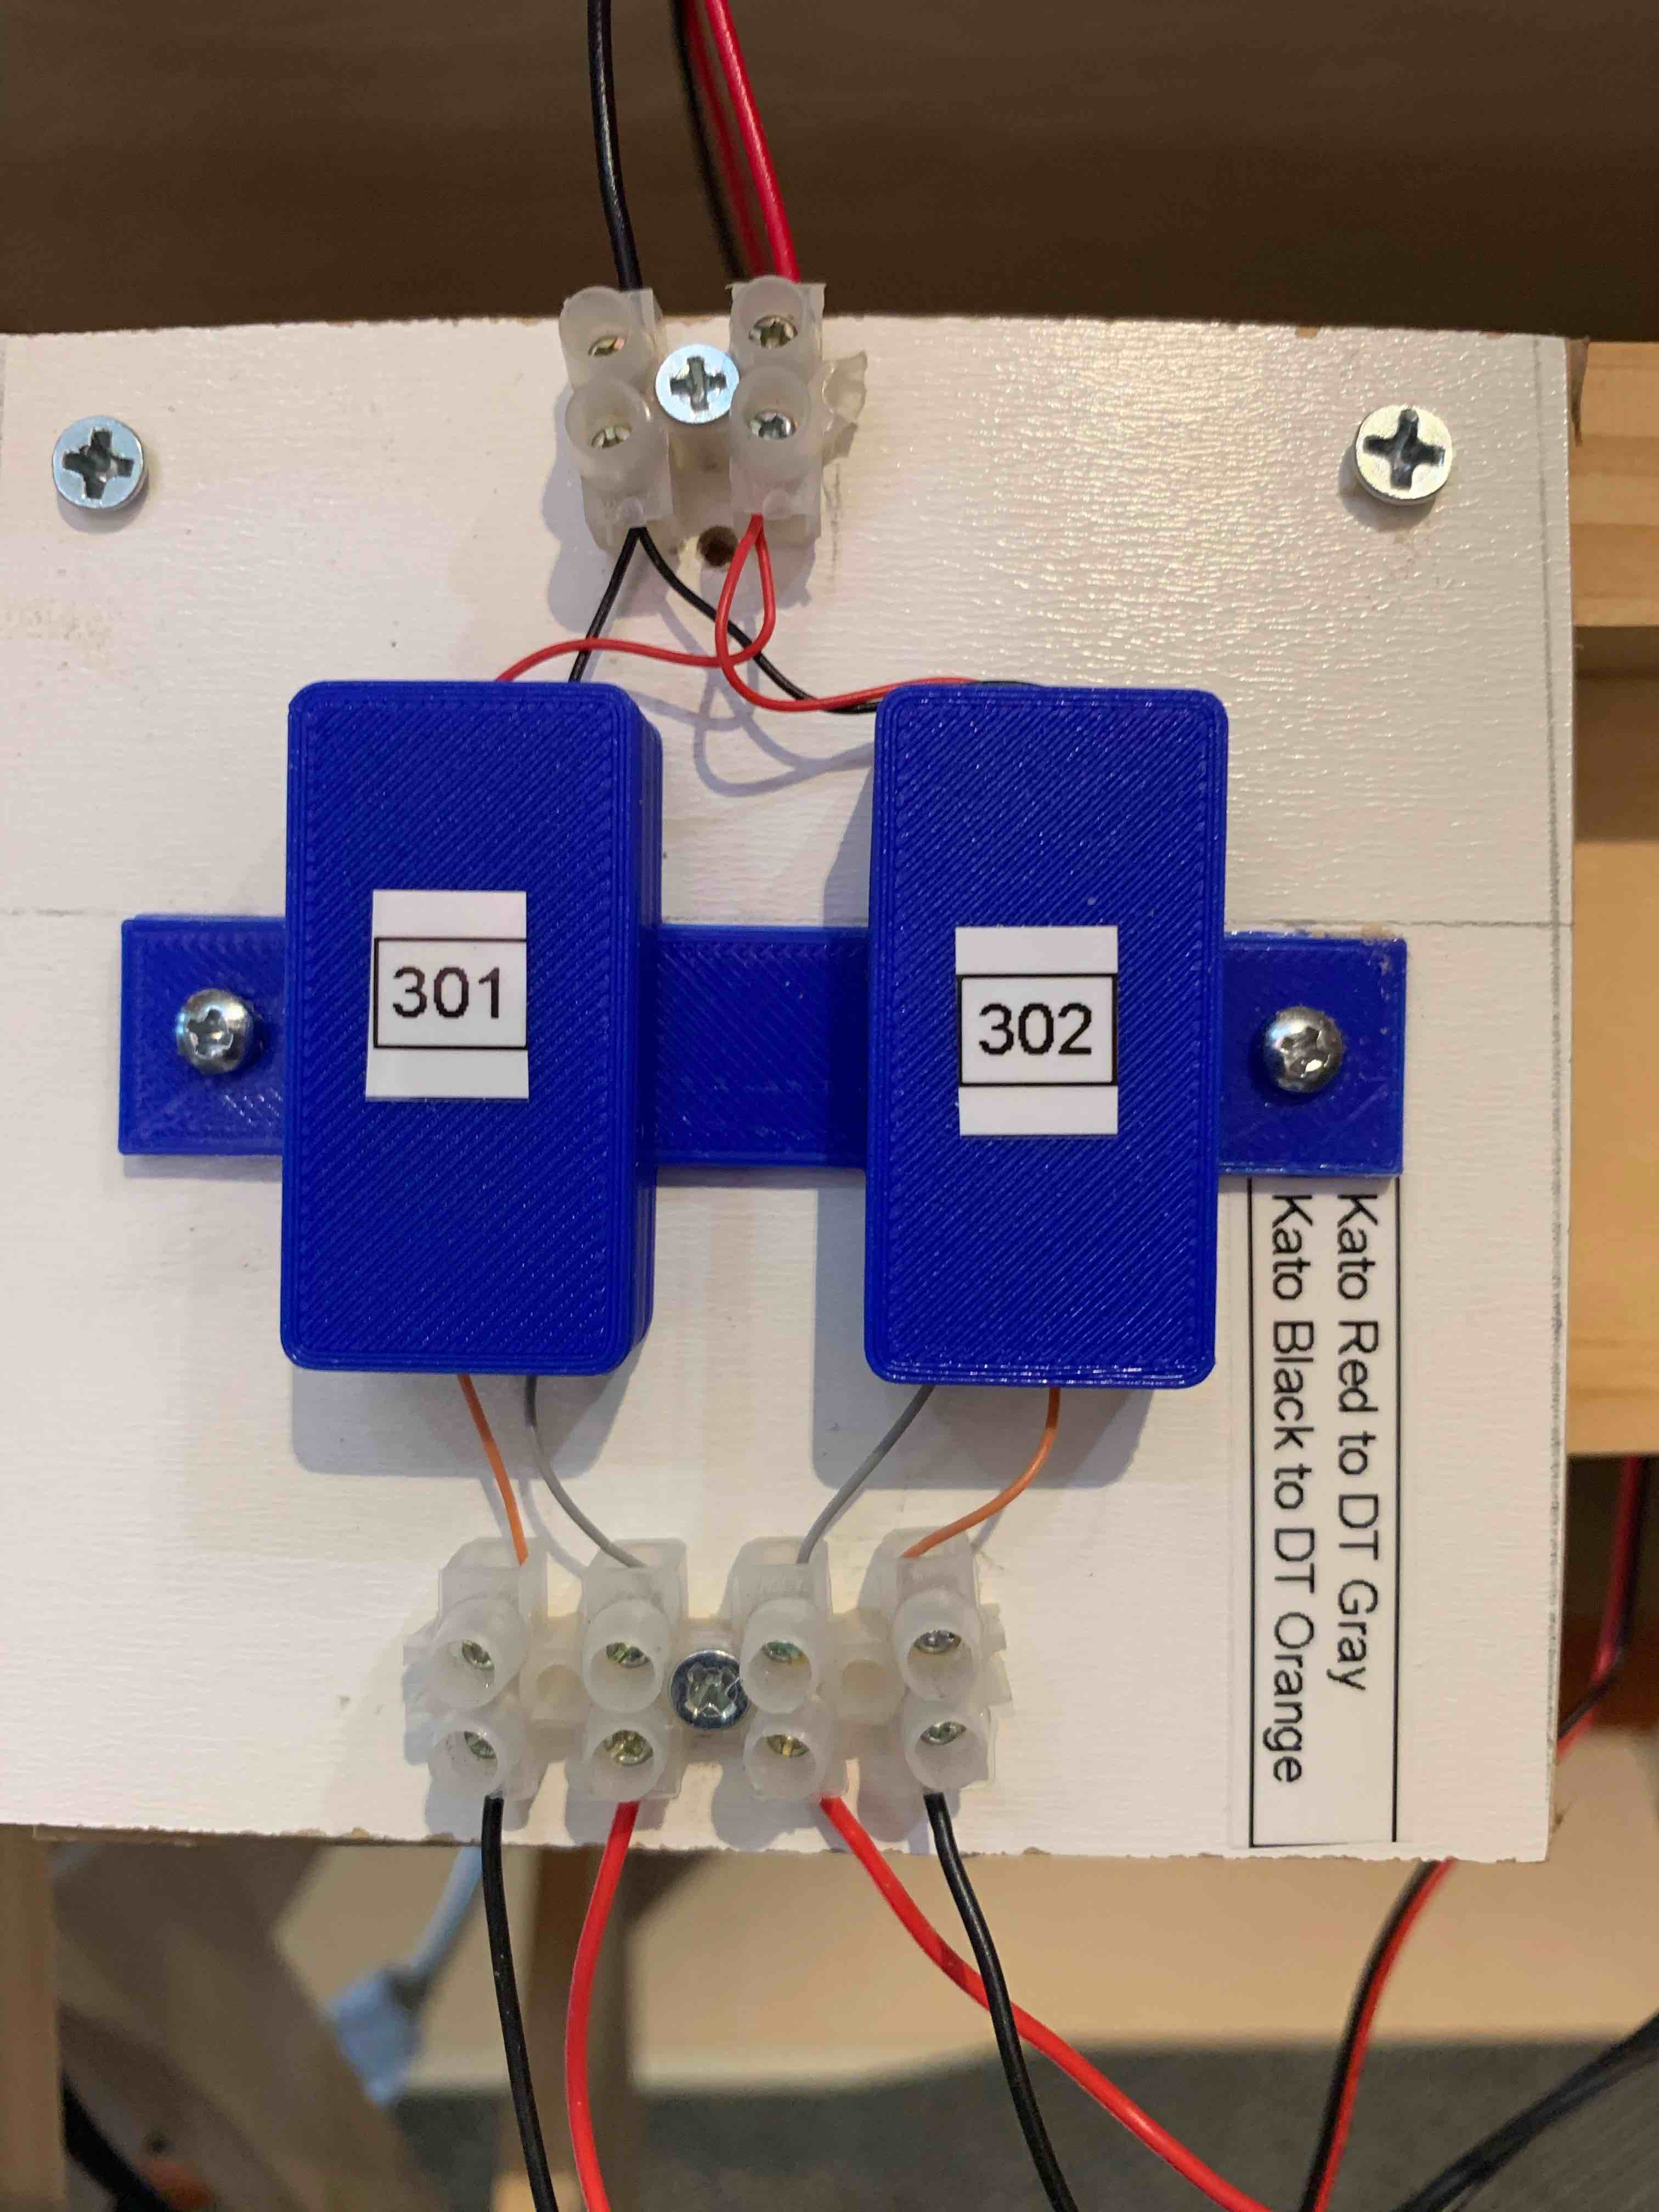
\includegraphics[width=0.475\textwidth]{./figures/printer/TwoBoxes.jpg}
           % \caption[Network2]%
           % {{\small Network 1}}    
            \label{fig:mean and std of net14}
        \end{subfigure}
        \hfill
        \begin{subfigure}[b]
            \centering 
            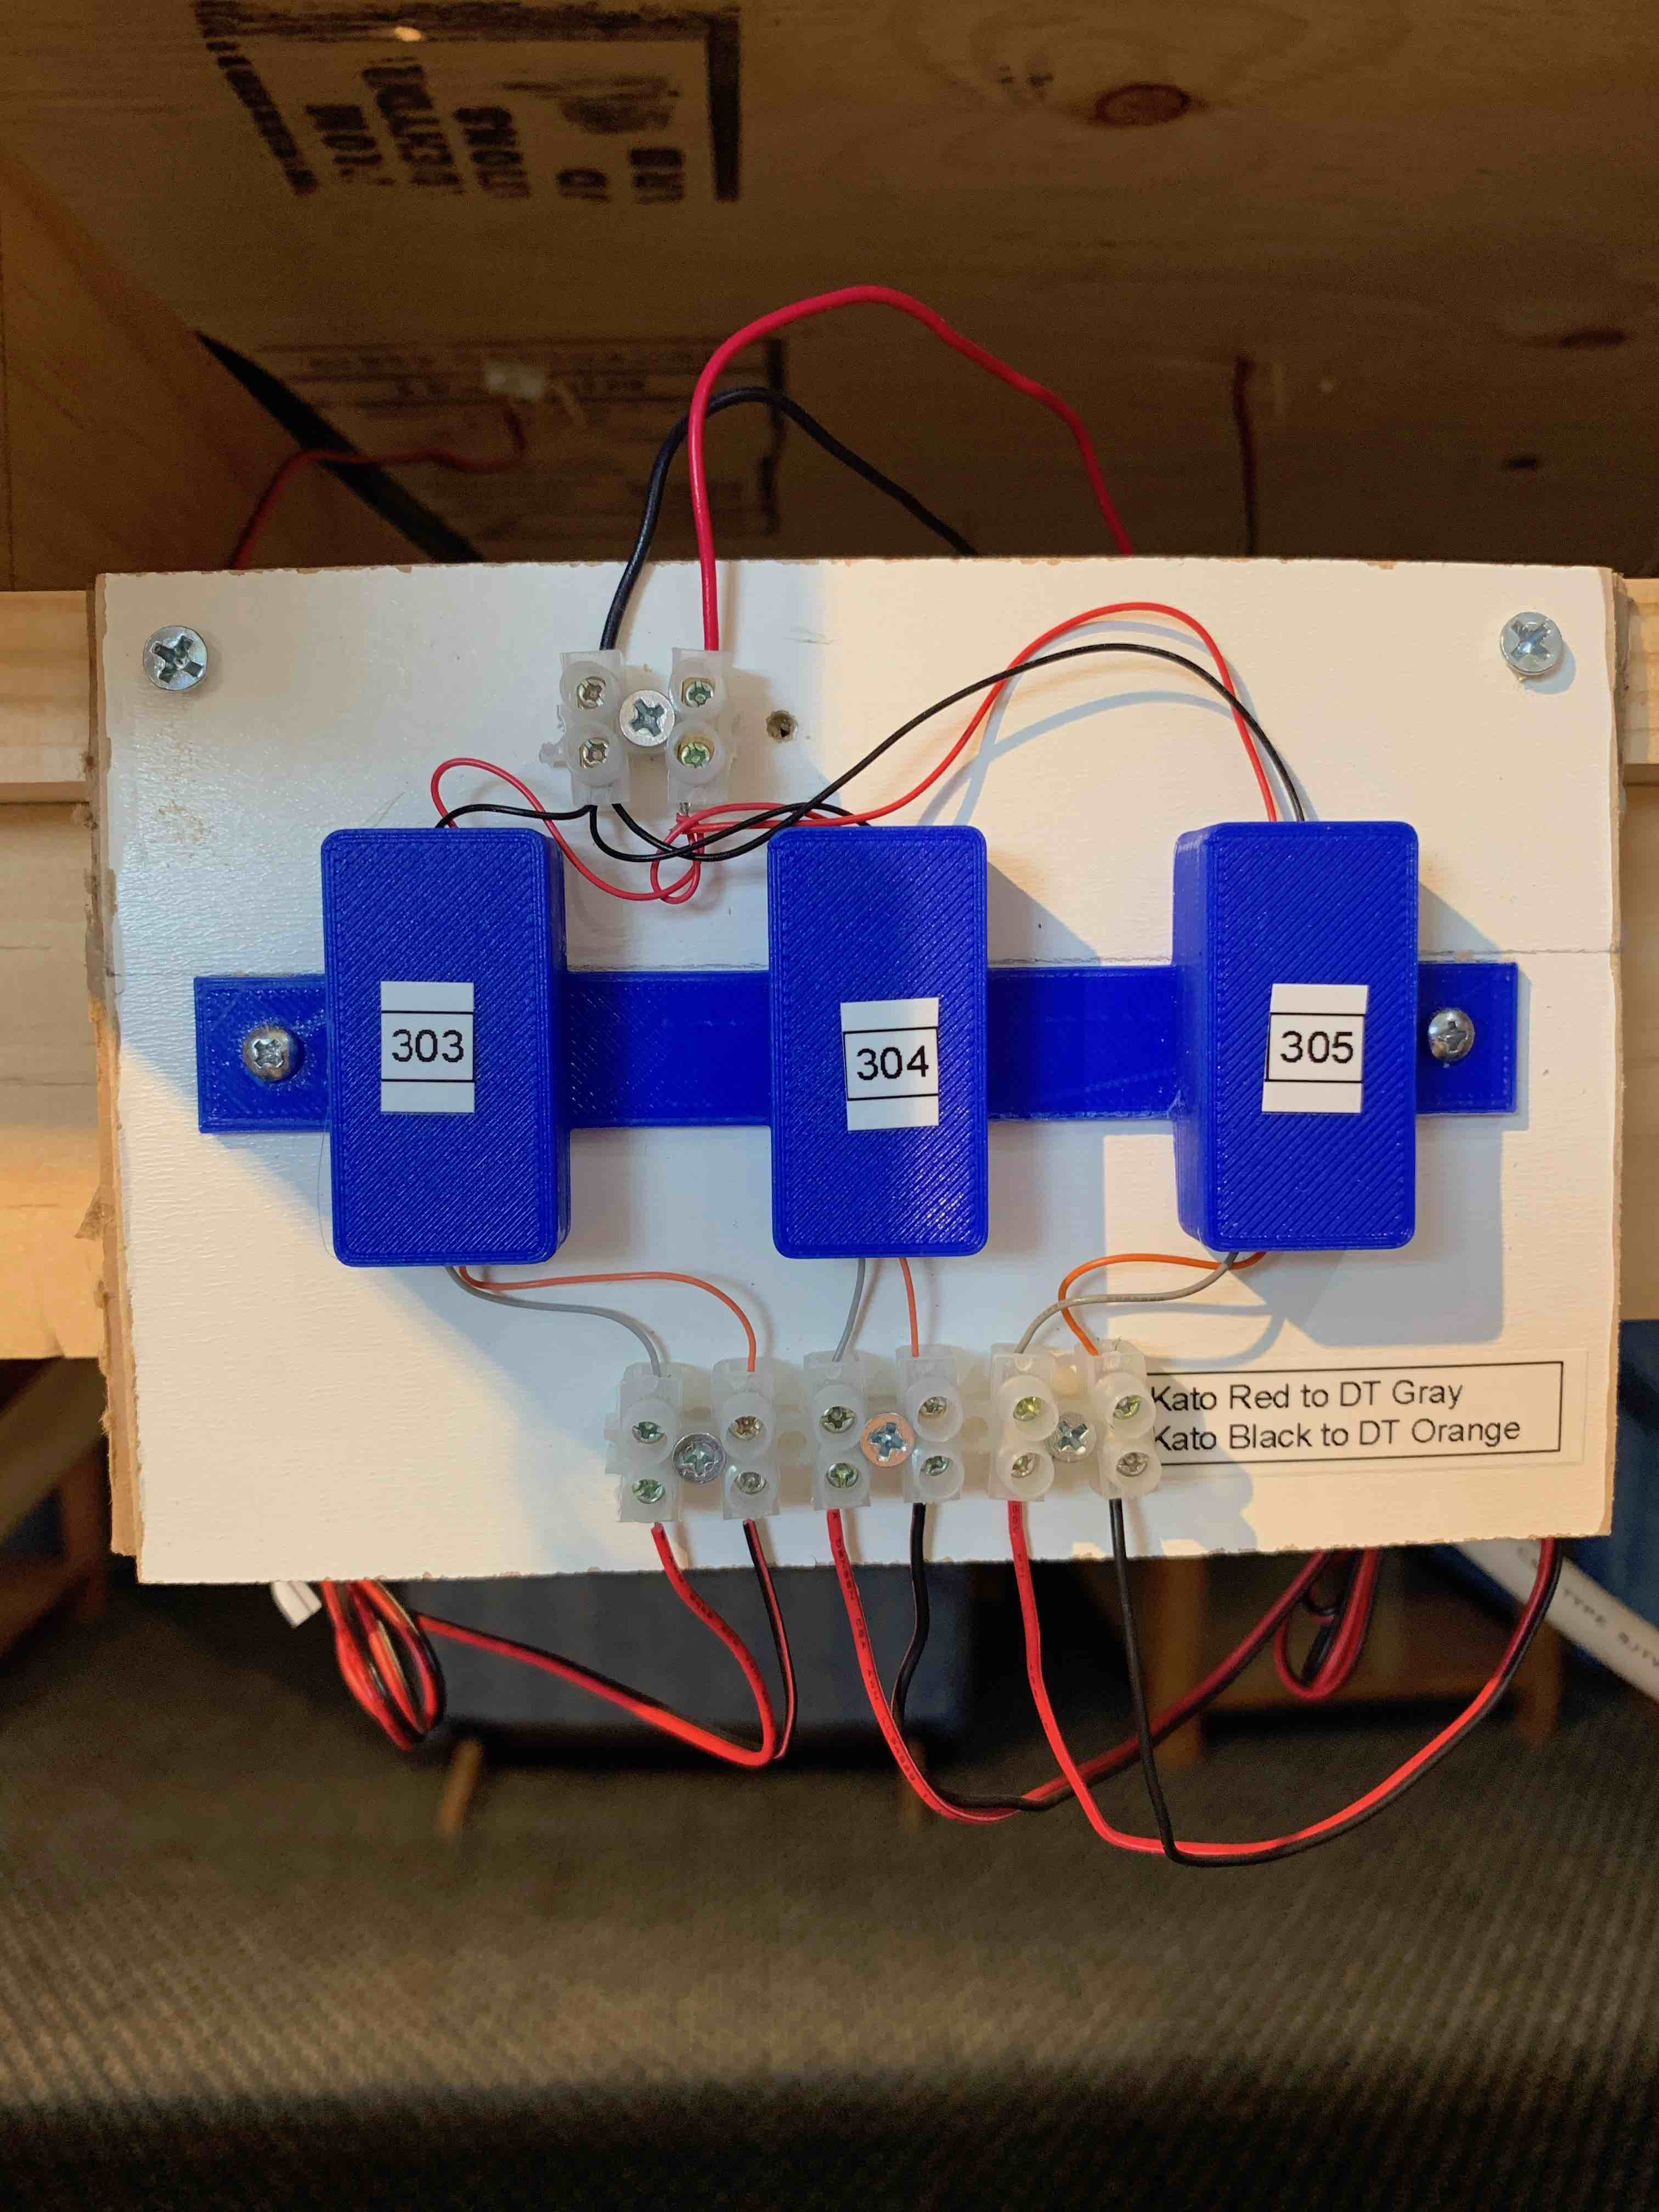
\includegraphics[width=0.475\textwidth]{./figures/printer/ThreeBoxes.jpg}
          %  \caption[]%
           % {{\small Network 2}}    
            \label{fig:mean and std of net24}
        \end{subfigure}
        \vskip\baselineskip
        \begin{subfigure}[b] 
            \centering 
            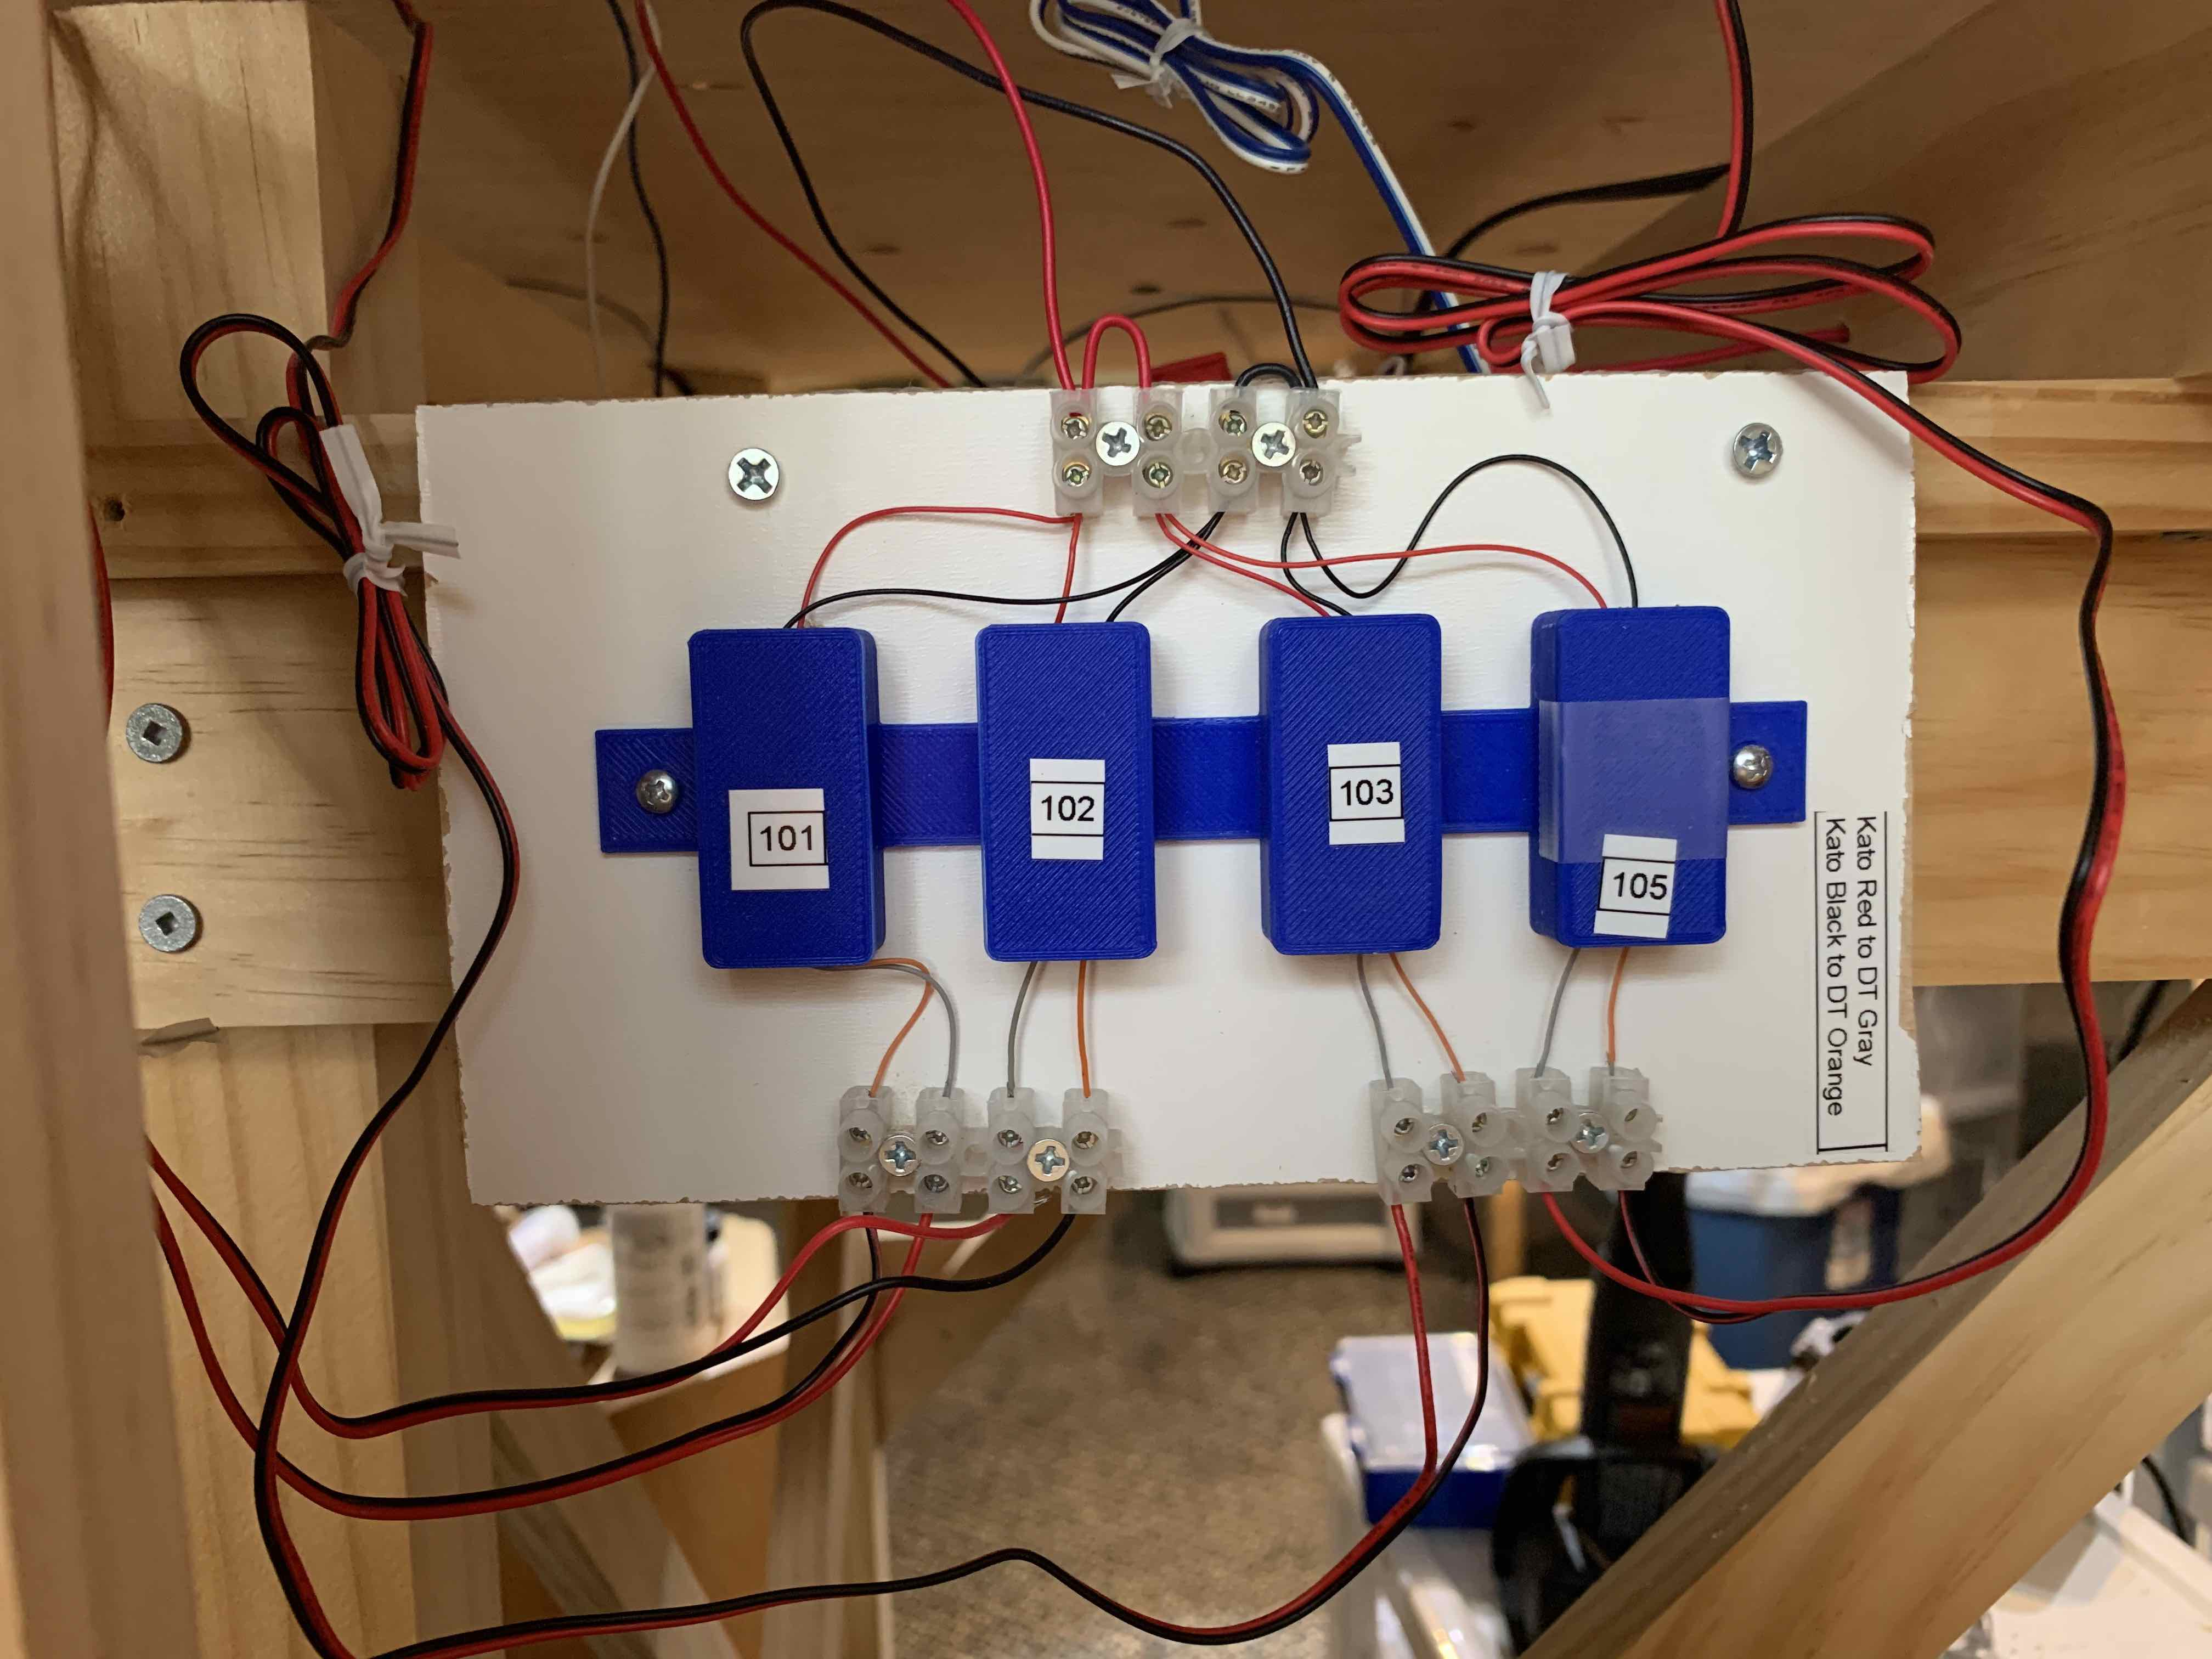
\includegraphics[width=0.475\textwidth]{./figures/printer/FourBoxes.jpg}
         %   \caption[]%
           % {{\small Network 3}}    
            \label{fig:mean and std of net34}
        \end{subfigure}
        \quad
        \begin{subfigure}[b]  
            \centering 
            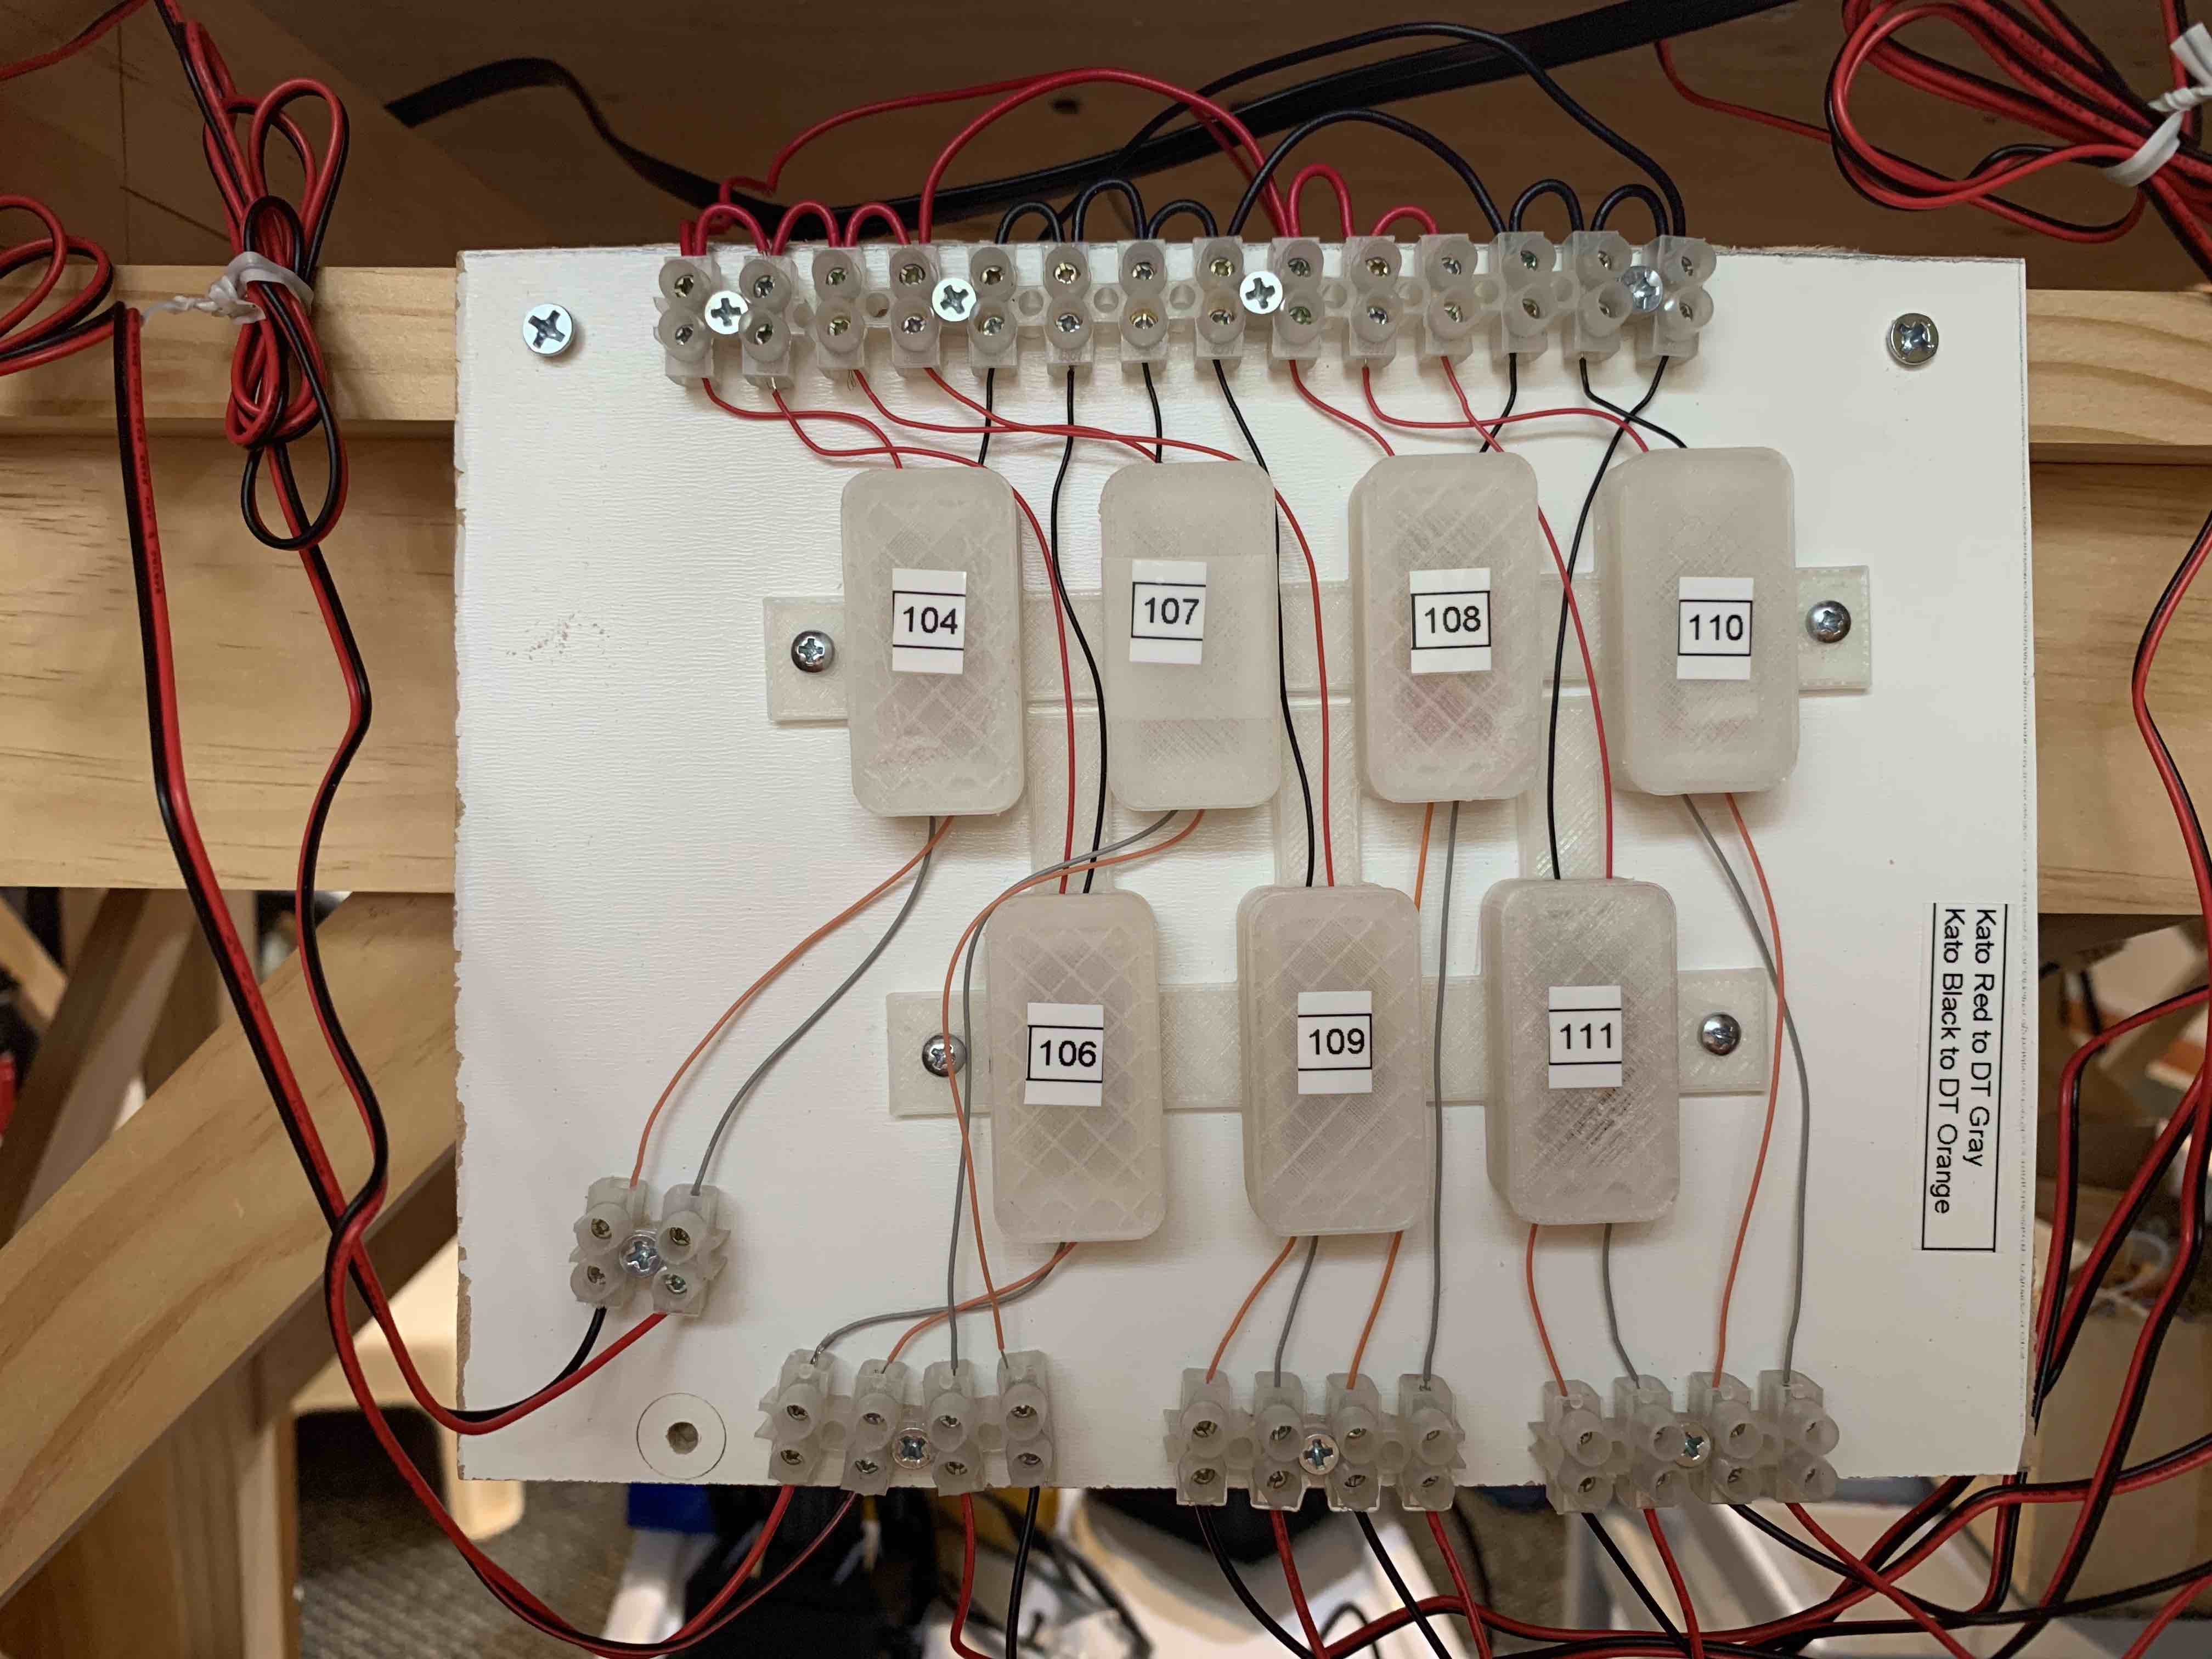
\includegraphics[width=0.475\textwidth]{./figures/printer/SevenBoxes.jpg}
          %  \caption[]%
           % {{\small Network 4}}    
            \label{fig:mean and std of net44}
        \end{subfigure}
        \caption[ The average and standard deviation of critical parameters ]
        {\small The average and standard deviation of critical parameters: Region R4} 
        \label{fig:mean and std of nets}
    \end{figure*}
    
